When having to compose concurrent systems we define three different semantics that can be applied pairwise. Synchronous semantic $A ||_s B$ (Figure~\ref{fig:synchronous_composition})captures the composition of two components that share a single synchronizing event (implicit), where all participants should be able to make progress concurrently. The main motivation being digital components sharing a single clock. 
Asynchronous semantic $A ||_a B$ (Figure~\ref{fig:asynchronous_composition}) captures the interleaving interpretation of concurrency as found in LTS systems. 

\begin{figure}[h]
		\centering
	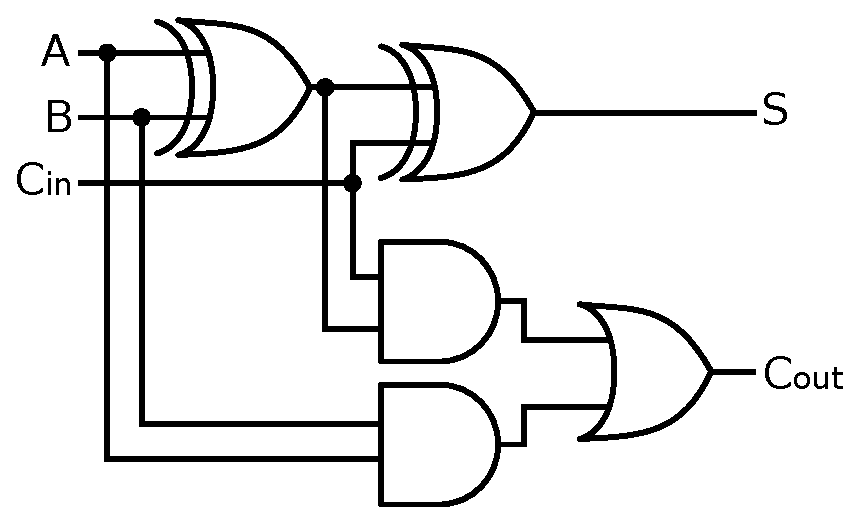
\includegraphics[scale=.4]{img/full-adder.eps}
	\caption{Full adder circuit}
	\label{fig:full_adder_circuit}
\end{figure}

A motivation for the synchronous composition can be found in the following example: a digital design consists of two 1 bit full adders working as separate units. Let $i \in \{1,2\}$ be the index of each adder and $a$ and $b$ the 1 bit entries to be added, $c\_in_i$ the incoming carry signal from another module, $s_i$ the output that represents the lower bit of the sum and $c_i$ the upper bit or carry out, then each 1 bit full adder can be modeled as a single state CLTS.  The FSP syntax would be the following:

\renewcommand{\ttdefault}{pcr}
\begin{figure}[H]
	\begin{lstlisting}[escapeinside={[*}{*]},basicstyle=\scriptsize\ttfamily,columns=flexible,mathescape=true,xleftmargin=3.0ex,keywordstyle=\textbf,morekeywords={if,while,do,else,fork,int,null, algorithm, is, input, output, return, for}]
	FULL_ADDER[i] = (<a[i],s[i]> -> FULL_ADDER[i] | <b[i],s[i]> -> FULL_ADDER[i] 
	| <c_in[i],s[i]> -> FULL_ADDER [i] | <a[i],b[i],c[i]> -> FULL_ADDER[i]
	| <a[i],c_in[i],c[i]> -> FULL_ADDER[i] | <b[i],c_in[i],c[i]> -> FULL_ADDER[i]
	| <a[i],b[i],c_in[i],s[i],c[i]> -> FULL_ADDER[i]| <> -> FULL_ADDER[i]).
\end{lstlisting}
%\caption{Game Structure to CLTS translation algorithm}
\label{fig:full_adder_fsp}
%%\vspace*{-4mm}
\MediumPicture
\end{figure}	

Applying asynchronous composition over single element labeled CLTS models ($FULL\_ADDER[1]$ $\parallel_{a}$ $FULL\_ADDER[2]$), would not properly capture the concurrent occurrence of signals, since it will not allow $<a_1,s_1,a_2,s_2>$ to happen.  

On the other hand, suppose that we are modeling the interaction of three processes $P_1$, $P_2$ and $receiver$ through a common buffer, $P_1$ produces either $a$ or $c$ and
$P_2$ produces either $d$ or $e$. $receiver$ will output a $x$ for each $a$ and a $y$ for each $d$. The FSP syntax would be the following:

\renewcommand{\ttdefault}{pcr}
\begin{figure}[H]
	\begin{lstlisting}[escapeinside={[*}{*]},basicstyle=\scriptsize\ttfamily,columns=flexible,mathescape=true,xleftmargin=3.0ex,keywordstyle=\textbf,morekeywords={if,while,do,else,fork,int,null, algorithm, is, input, output, return, for}]
	P_1 = (a->P_1 | c->P_1).
	P_2 = (d->P_2 | e->P_2).
	Receiver = (<a,x> -> Receiver | <d,y> -> Receiver | c -> Receiver | e -> Receiver).
	\end{lstlisting}
	%\caption{Game Structure to CLTS translation algorithm}
	\label{fig:receiver_fsp}
	%%\vspace*{-4mm}
	\MediumPicture
\end{figure}

Special attention is required when applying the parallel composition operator in order to recreate the system overall interaction. If synchronous semantic ($P_1\parallel_s P_2 \parallel_s receiver$) is to be applied then $receiver$ will not be able to synchronize with both $P_1$ and $P_2$ since at least one action on each component needs to be exercised. In this case, asynchronous composition ($P_1\parallel_a P_2 \parallel_a receiver$)will properly recreate the serialization of events coming from $P_1$ and $P_2$ through the buffer.

Composition semantics should be applied according the each domain, be aware that composition is not commutative if different semantics are applied for the same specification.
